\documentclass[11pt, a4paper]{article}
\usepackage[utf8]{inputenc}
\usepackage{graphicx}
\usepackage{geometry}
\usepackage{hyperref}
\usepackage{xcolor}
\usepackage{titlesec}
\usepackage{booktabs}
\usepackage{enumitem}

\geometry{a4paper, margin=1in}
\titleformat{\section}{\large\bfseries\color{blue!70!black}}{\thesection}{1em}{}
\titleformat{\subsection}{\normalsize\bfseries\color{black!80}}{\thesubsection}{1em}{}
\setlist[itemize]{leftmargin=*}

\title{\vspace{-1.5cm}\textbf{Proposal for Production Adoption:\\Dynamic Vector Search Allocation via \texttt{shiro-ef}}}
\author{Research \& Engineering}
\date{\today}

\begin{document}
\maketitle

\begin{abstract}
This proposal advocates for the integration of \texttt{shiro-ef}, a dynamic effort-allocation algorithm, into our production vector search pipelines. Currently, our infrastructure suffers from a massive ``noise tax''. Because standard search algorithms use a fixed search depth, we are forced to over-provision compute for trivial queries just to ensure we don't fail on complex, high-value user requests. \texttt{shiro-ef} solves this by dynamically halting search early for easy queries and reallocating that compute budget exclusively to difficult ones. Empirical results show that \texttt{shiro-ef} maintains premium accuracy for edge cases while slashing overall median latency by nearly 40\%, offering a massive reduction in cloud infrastructure costs and a significantly faster experience for the majority of our users.
\end{abstract}

\section{The Fundamental Problem: The "Noise Tax"}
In production retrieval systems, the difficulty of incoming user queries is highly skewed. The vast majority of traffic consists of straightforward, ``noisy'' queries that are trivial to answer. A small, crucial minority consists of complex, ``hard'' queries that require deep database traversal.

Because standard vector databases (like HNSW) rely on a \textbf{fixed, one-size-fits-all parameter} (such as $efSearch$), engineering teams face an expensive dilemma. To ensure we successfully answer the complex, high-value queries, we are forced to set a massive global search depth ($EF=500$). We continuously burn enormous amounts of expensive cloud CPU endlessly over-searching trivial queries, simply as an insurance policy to protect the complex queries.

\section{Comprehensive Real-World Business Cases}
To understand the scope of the ``Noise Tax'' and how \texttt{shiro-ef} resolves it, consider how query difficulty varies across our core business verticals:

\subsection{1. Enterprise AI and RAG (Retrieval-Augmented Generation)}
\begin{itemize}
    \item \textbf{The Easy Query (80\%):} \textit{``How do I reset my company password?''} The answer exists in dozens of IT FAQs. Any shallow search will retrieve it in sub-milliseconds.
    \item \textbf{The Hard Query (10\%):} \textit{``Why does error 0x800A trigger during v2 API syncs on legacy Windows clients?''} The exact answer is buried in a single Slack thread from three years ago. 
    \item \textbf{The \texttt{shiro-ef} Impact:} Prevents the AI from hallucinating on critical engineering questions by digging deep, while preventing the chatbot from wasting GPU/CPU tokens over-thinking basic HR queries.
\end{itemize}

\subsection{2. E-Commerce and Retail Search}
\begin{itemize}
    \item \textbf{The Easy Query (80\%):} \textit{``Black Nike running shoes.''} There are millions of acceptable, highly relevant matches.
    \item \textbf{The Hard Query (10\%):} \textit{``Waterproof zero-drop trail running shoes for men with plantar fasciitis under \$100.''} A highly specific, long-tail query with multiple constraints.
    \item \textbf{The \texttt{shiro-ef} Impact:} Protects conversion rates for high-intent, niche buyers by finding the exact product, while saving AWS costs on users doing generic window-shopping.
\end{itemize}

\subsection{3. Content Recommendation (Feeds \& Streaming)}
\begin{itemize}
    \item \textbf{The Easy Query (80\%):} Generating a feed for a new user, or suggesting a globally viral entertainment video.
    \item \textbf{The Hard Query (10\%):} Suggesting a video on \textit{``18th-century Japanese woodworking techniques''} to a power user with deeply established, specific niche interests.
    \item \textbf{The \texttt{shiro-ef} Impact:} Drives long-term user retention for niche communities, without bottlenecking the recommendation engine when building generic feeds for the masses.
\end{itemize}

\subsection{4. Cybersecurity and Fraud Detection}
\begin{itemize}
    \item \textbf{The Easy Query (80\%):} Recognizing a known, blatant phishing IP pattern or a standard brute-force login attack.
    \item \textbf{The Hard Query (10\%):} Detecting subtle, zero-day Advanced Persistent Threat (APT) behavior that has been deliberately obfuscated to only vaguely resemble known vectors.
    \item \textbf{The \texttt{shiro-ef} Impact:} Ensures security analysts do not miss sophisticated, buried attacks, while standard network traffic is processed instantly without bogging down the SIEM.
\end{itemize}

\section{The Proposed Solution: \texttt{shiro-ef}}
\texttt{shiro-ef} eliminates this infrastructure waste by acting as an intelligent load-balancer on the fly:
\begin{enumerate}
    \item \textbf{Early Halting for Trivial Queries:} When handling generic queries (like the password reset or black running shoes), it aggressively halts the search early, delivering the result instantly and freeing up the CPU.
    \item \textbf{Targeted Investment for Complex Queries:} When a query is highly specific and struggling to find matches, \texttt{shiro-ef} reallocates the saved compute budget exclusively toward these hard queries, guaranteeing we don't lose the sale, hallucinate the answer, or miss the security threat.
\end{enumerate}

\section{Experimental Evidence}
We benchmarked \texttt{shiro-ef} against our heavy production baseline ($EF=500$). Sorting the queries from hardest to easiest reveals three distinct operational zones:
\begin{itemize}
    \item \textbf{The Investment (Hardest $\sim$27\%):} \texttt{shiro-ef} deliberately invests higher latency into complex, niche queries. This rescues them from failure, boosting their recall up to highly respectable levels.
    \item \textbf{The Breakeven (Medium $\sim$10\%):} The algorithm seamlessly transitions, spending identical latency to achieve identical accuracy as the baseline.
    \item \textbf{The Profit (Easiest $\sim$63\%):} For the generic majority, \texttt{shiro-ef} drastically cuts latency. Stopping early costs practically zero accuracy (maintaining near-perfect $1.0$ recall).
\end{itemize}

% \begin{figure}[h]
% \centering
% % 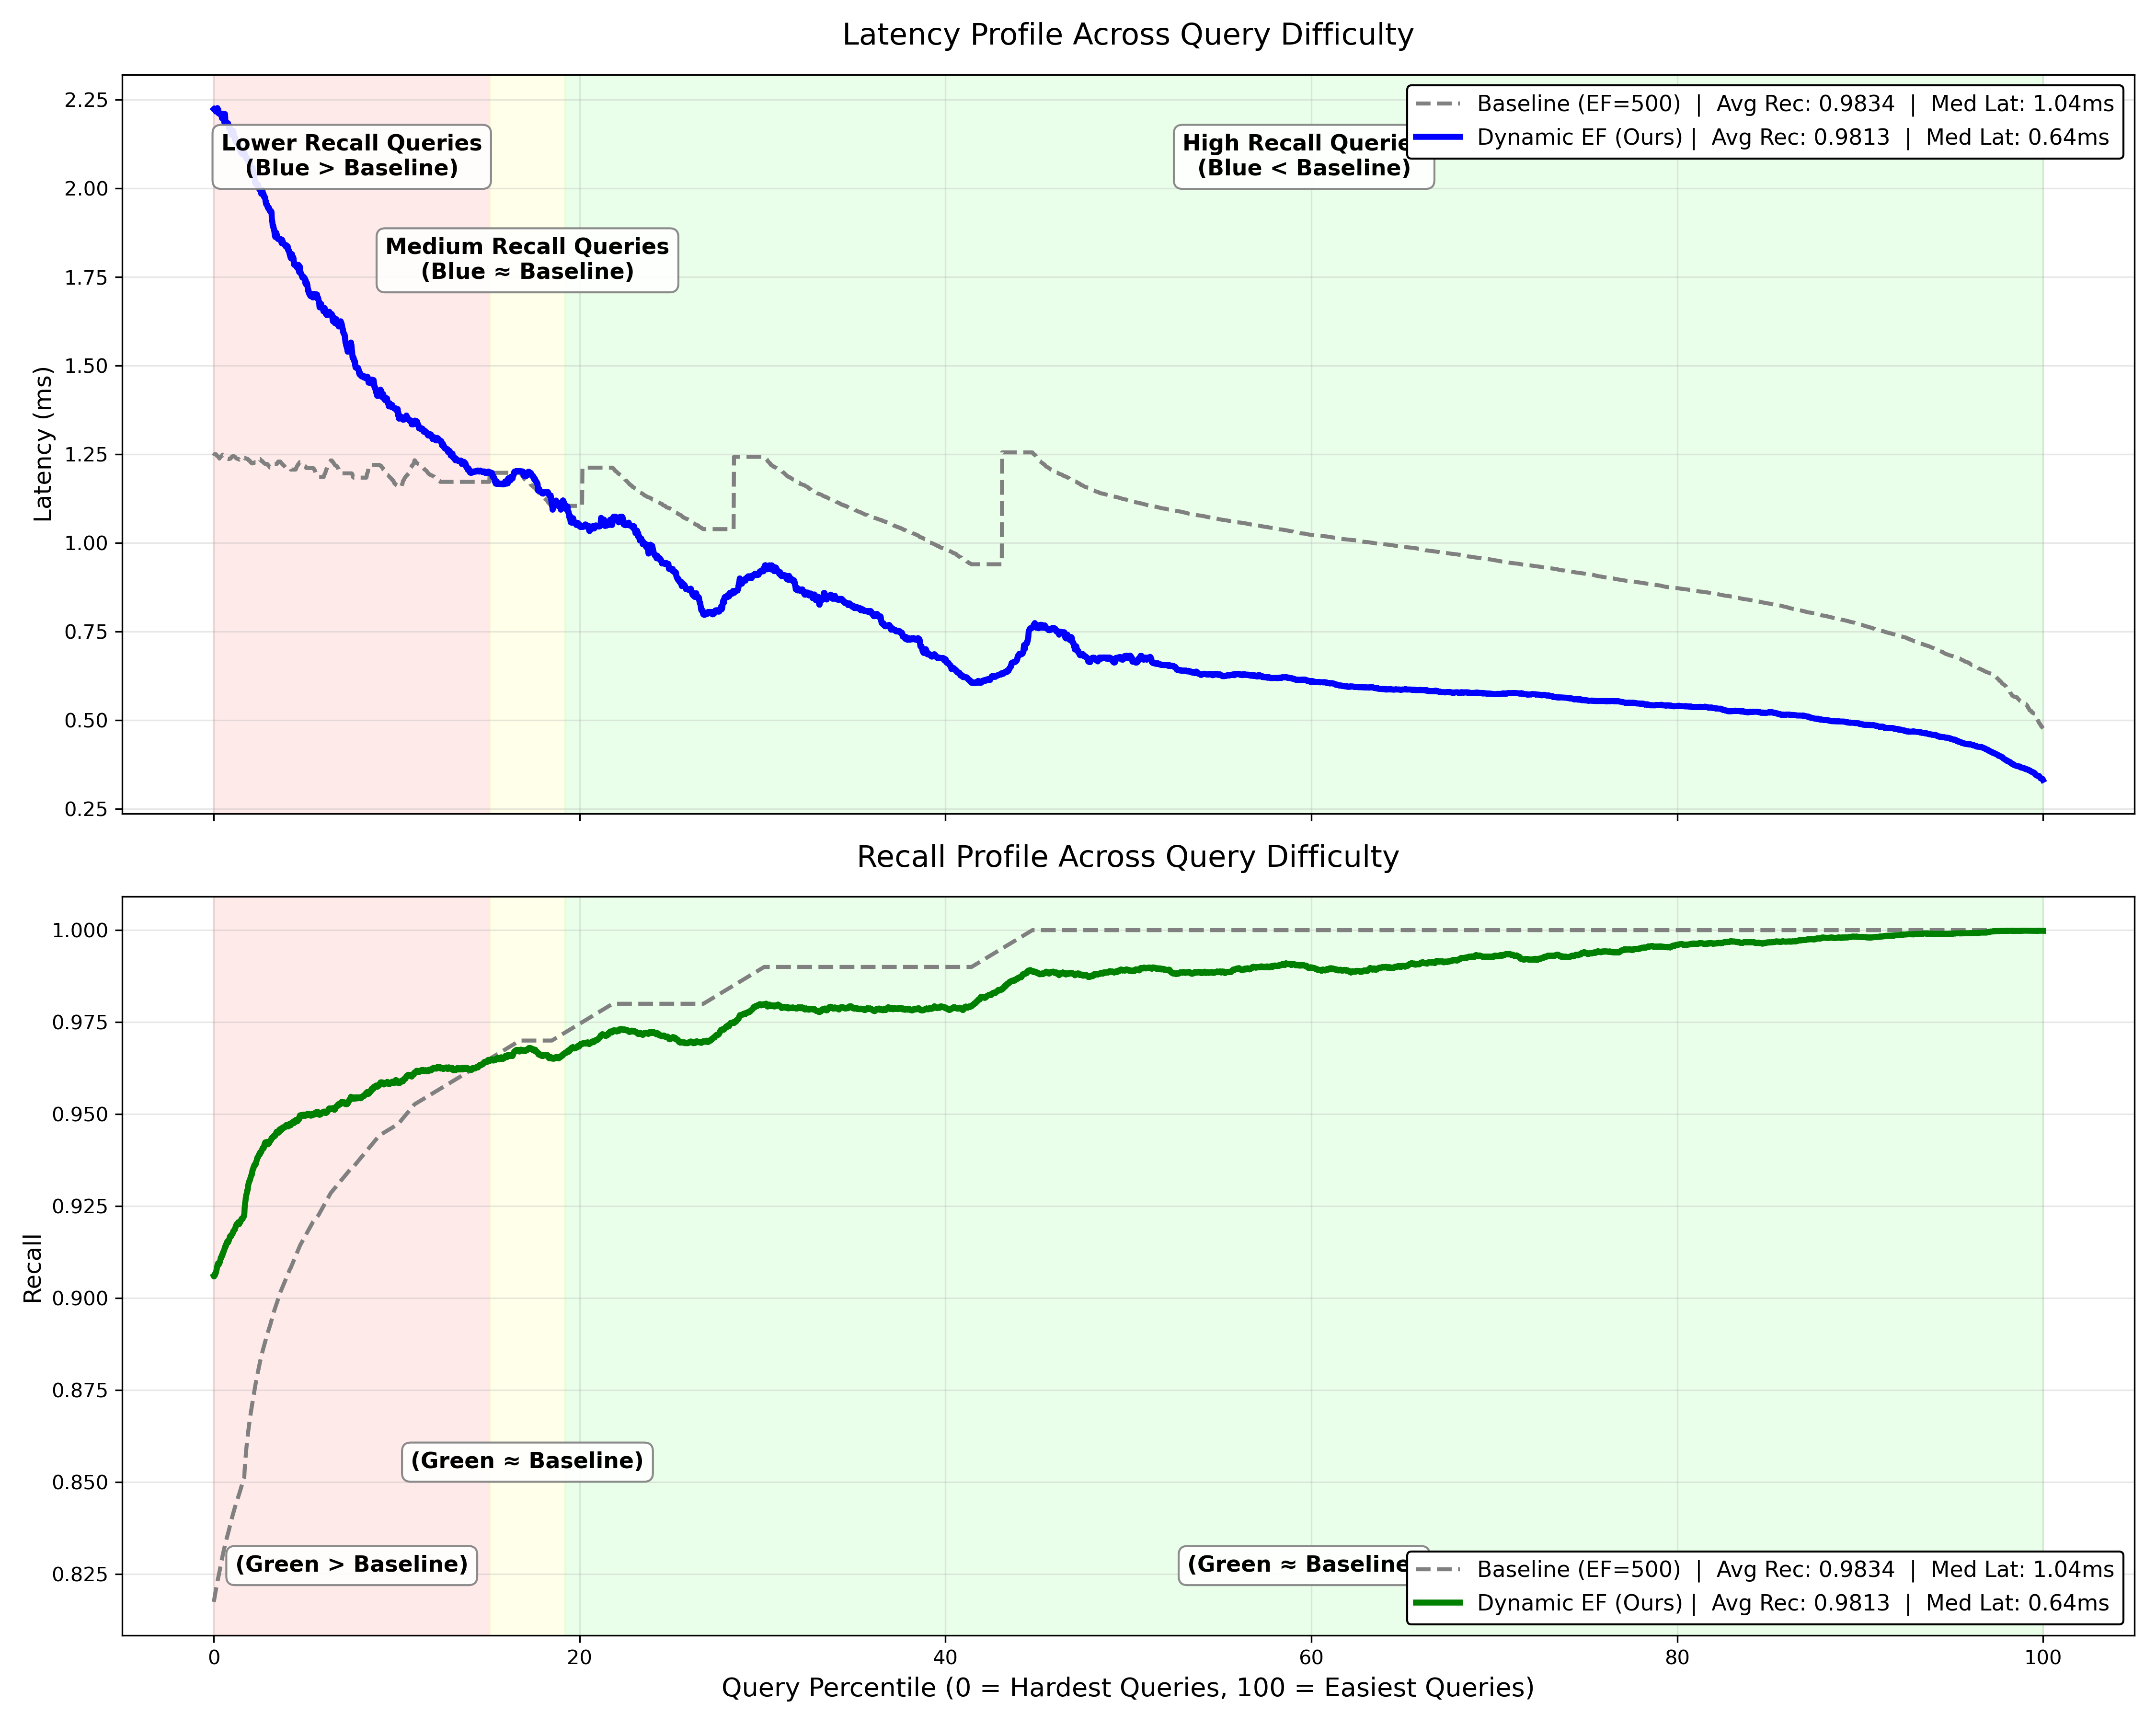
\includegraphics[width=0.95\textwidth]{csv/story_continuous_final.png}
% \caption{Latency and Recall Profile across Query Difficulty. \texttt{shiro-ef} effectively reallocates wasted latency from the right side (Easy queries) to the left side (Hard queries).}
% \label{fig:performance}
% \end{figure}

\section{Business Impact and Conclusion}
The adoption of \texttt{shiro-ef} into our core retrieval pipelines offers a clear, high-leverage Return on Investment (ROI):
\begin{itemize}
    \item \textbf{Massive Infrastructure Cost Savings:} By stopping early on the 63\% of easy queries, we slash overall median latency by \textbf{38.5\%} (dropping from 1.04ms down to 0.64ms). This directly translates to lower CPU utilization, allowing us to handle more traffic on fewer servers.
    \item \textbf{Faster User Experience:} 80\% of users (and automated systems) will receive results noticeably faster.
    \item \textbf{Protected Revenue and Quality:} We secure the premium, high-accuracy recall of a brute-force search for the complex, long-tail queries that actually drive specialized revenue and rely on exact matches.
\end{itemize}

I propose that we begin integration testing of \texttt{shiro-ef} into the staging environment for our primary vector databases.

\end{document}
